\documentclass{article}
\usepackage[utf8]{inputenc}
\usepackage[italian]{babel}
\usepackage{graphicx}
\usepackage{xcolor}
\usepackage[a4paper,top=15mm, bottom=15mm, left=15mm, right=15mm]{geometry}
\usepackage{listings}
\usepackage{subfig}

\begin{document}
	
	\title{Algoritmi e diagrammi di flusso}
	\author{Alessandro Fuser}
	\maketitle
	
	\pagebreak
	
	\tableofcontents
	
	\pagebreak
	
	\section{Teoria}
	\subsection{Gli algoritmi}
	Un \textbf{algoritmo} è la descrizione del percorso risolutivo di un problema per giungere dai dati iniziali ai risultati finali. Questo viene scritto pensando di rivolgersi a un \textbf{esecutore}, capace di svolgere azioni descritte da \textbf{istruzioni}, scritte in un particolare \textbf{linguaggio}.\\
	Un'altra possibile definizione di algoritmo è la seguente: "Un algoritmo è un procedimento di calcolo che si basa sull'applicazione di un numero finito di regole che determinano in modo meccanico TUTTI i singoli passi del procedimento stesso". In parole più brevi, potremmo definirlo come ogni procedimento che consente di risolvere un problema.\\
	L'algoritmo è un concetto fondamentale dell'informatica, anzitutto perché è alla base della nozione teorica di calcolabilità, in quanto un \textbf{problema è calcolabile solo quando è risolvibile mediante un algoritmo}. Se ci pensate, usiamo algoritmi tutti i giorni per risolvere ogni tipo di problema che ci si presenta davanti.
	
	Le principali operazioni presenti all'interno di un algoritmo sono:\\
	\begin{center}
		\begin{tabular}[h!]{|c|c|}
			\hline
			Istruzioni di & Per \\ \hline
			\textbf{Input} & Ricevere dati (numeri, espressioni, testi) \\ \hline
			\textbf{Output} & Mandare messaggie  comunicare risultati \\ \hline
			\textbf{Assegnazione} & Memorizzare un dato associandolo al nome di una variabile \\ \hline
			\textbf{Calcolo} & Svolgere operazioni tra i dati \\
			\hline
		\end{tabular}
	\end{center}
	Quando mi serve salvare un qualche valore o dato, posso fare uso di una variabile. Una \textbf{variabile} è un contenitore di dati destinato a contenere dei valori, che può essere modificata durante l'esecuzione di un programma. Ad esempio, se voglio salvare l'informazione che un lato di un rettangolo ha valore 10, allora mi basta assegnare tale valore ad una variabile, che avrà un proprio nome, del tipo:\\
	\begin{center}
		cateto = 10;\\
		base = 15;\\
		altezza = 5;
	\end{center}
	Certe variabili non vengono assegnate direttamente dall'utente, ma vengono prodotte nell'esecuzione di un programma. Pensa ad esempio al calcolo dell'area di un rettangolo. Per fare tale operazione, ti servirà il valore della base e dell'altezza del rettangolo (che salverai in apposite variabili) e, per salvare il valore dell'area, userai una nuova variabile, del tipo:\\
	\begin{center}
		area = base * altezza;\\
		perimetro = (base + altezza) * 2;
	\end{center}
	\begin{large}
	\textcolor{red}{Quando vuoi salvare un valore per poterlo usare successivamente all'interno di un programma, salvalo in una variabile, di cui decidi tu il nome}.
	\end{large}\\
	I tipi principali che una variabile può assumere sono:\\
	\begin{center}
		\begin{tabular}[h!]{|c|c|}
			\hline
			Tipo & Per \\ \hline
			\textbf{int} & Numeri interi (0, 1, 3, ...) \\ \hline
			\textbf{double} & Numeri con la virgola o frazionari \\ \hline
			\textbf{string} & Parole o lettere \\ \hline
			\textbf{bool} & Valori vero o falso (1 e 0) \\ \hline
		\end{tabular}
	\end{center}
	\subsubsection{Proprietà degli algoritmi}
	Le proprietà principali di un algoritmo sono 5:\\
	\begin{center}
		\begin{tabular}{|c|c|}
			\hline
			Nome Proprietà & Descrizione \\ \hline
			Generale & Deve risolvere una classe di problemi e non un singolo problema \\ \hline
			Finito & Devo avere un numero ben preciso di passi da svolgere \\\hline
			Completo & Deve tenere conto di tutti i possibili casi da risolvere \\ \hline
			Non ambiguo & Ogni istruzione deve essere definita in modo preciso ed univoco \\ \hline
			Eseguibile & Deve esistere qualcuno o qualcosa che sia in grado di eseguire l'algoritmo \\ \hline
		\end{tabular}
	\end{center}
	Altre proprietà molto utili sono:
	\begin{itemize}
		\item \textbf{Modularità}, ossia la capacità di suddividere il problema generale in sotto-problemi più semplici;
		\item \textbf{Gerarchia}, ossia l'esistenza di un ordine ben specifico in cui le operazioni vengono svolte;
		\item \textbf{Realizzabilità}, ossia la capacità, da parte di chi legge l'algoritmo, di poterlo eseguire con quello che ha a disposizione;
		\item \textbf{Efficienza}, ossia la diversa velocità di esecuzione degli algoritmi a parità di compito svolto
	\end{itemize}
	Le tipologie di algoritmo, invece, possono essere principalmente due: \textbf{deterministico} se, per ogni istruzione, esiste un solo passo successivo possibile; \textbf{non deterministico} se contiene almeno un'istruzione che ammette più passi successivi. Una volta che verrano spiegate le strutte dell'algoritmo, questo concetto diverrà molto più chiaro ed immediato.
	\begin{figure}[h!]
		\centering
		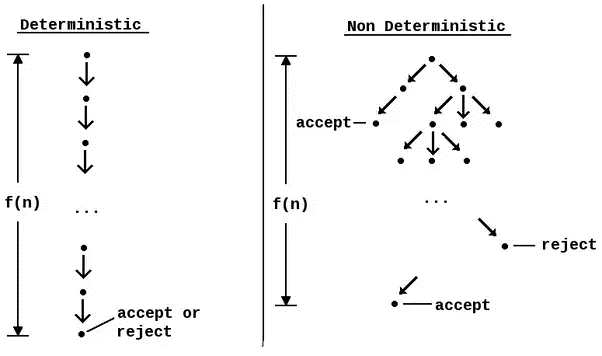
\includegraphics[scale=1]{Deterministico.png}
	\end{figure}
	\subsubsection{Esempi di algoritmo}
	Esempi di algoritmi scritti in linguaggio comune di tutti i giorni possono essere i seguenti: calcolo del perimetro di un rettangolo, misura di un catetto, massimo fra quattro numeri.\\
	Vediamo la risoluzione del \textbf{calcolo del perimetro di un rettangol}o:
	\begin{enumerate}
		\item Inizia
		\item Acquisisci il valore della base B e dell'altezza H
		\item Somma i valori di B e H ed assegnalo a P
		\item Raddoppia il valore di P ed assegnalo a 2P
		\item Rendi noto il valore di P
		\item Fine
	\end{enumerate}
	Risoluzione della \textbf{misura del cateto}:
	\begin{enumerate}
		\item Inizio
		\item Acquisisci l'ipotenusa A e il cateto B
		\item Controlla se A > B
		\item Se è vero, calcola $\sqrt{A^{2} - B^{2}}$ ed assegna il valore a C e rendi noto C
		\item Se è falso, scrivi un messaggio di errore
		\item Fine
	\end{enumerate}
	Risoluzione del \textbf{massimo fra quattro numeri}:
	\begin{enumerate}
		\item Inizio
		\item Leggi il primo numero e memorizzalo nella variabile M
		\item Ripeti la seguente operazione per 3 volte: leggi un numero e memorizzalo nella variabile N e se N è maggiore di M allora assegna il valore di N a M
		\item Rendi noto M
		\item Fine
	\end{enumerate}
	Esempio su un indovinello famoso, quello del \textbf{trasporto della capra, del lupo e del cavolo}: Un pastore ha una pecora, un lupo e un cavolo. Deve portarli dall'altra parte di un fiume che non ha né ponti né guadi, facendo ben attenzione che nel tragitto la pecora non sbafi il cavolo o - peggio - il lupo non sbrani la pecora. Il pastore ha a disposizione una piccola canoa che può contenere solo una cosa o un animale oltre al pastore. Quindi non è possibile fare il trasbordo in un unica soluzione .  Non ha nessun problema a far avanti e indietro nel fiume, ma si deve, invece,  fare attenzione anche a cosa combinano i due rimasti soli sulla riva mentre il pastore è in acqua con il terzo. Come fa il pastore a trasportare pecora, cavolo e lupo, tutti e tre sani, salvi e... non mangiati?
	\begin{enumerate}
		\item Porta la capra sull'altra sponda
		\item Torna indietro da solo
		\item Porta il cavolo dall'altra parte e carica la pecora
		\item Porta la capra indietro
		\item Scarica la capra e porta il lupo sull'altra sponda
		\item Torna indietro da solo
		\item Porta la capra sull'altra sponda
	\end{enumerate}	
	\subsubsection{Sequenza}
	Purtroppo, le macchine (computer) che non capiscono il linguaggio naturale usato dagli essere umani, per cui bisogna usare un linguaggio più definito e coinciso, senza possibilità di ambiguità.\\
	Usano un linguaggio più appropriato, dunque, possiamo risolvere il problema del calcolo del perimetro di un rettangolo nel seguente modo:\\
	\begin{lstlisting}
	Inizio
	SCRIVI "Fornisci la misura della base B"
	LEGGI B
	SCRIVI "Fornisci la misura dell'altezza H"
	LEGGI H
	P:= B+H
	2P:= 2*P
	SCRIVI "La misura del perimetro: "
	SCRIVI P
	Fine
	\end{lstlisting}
	Notiamo i seguenti fatti, che \textbf{valgono come regola generale} quando si scrive un algoritmo:
	\begin{itemize}
		\item Con il simbolo := si indica l'assegnazione di un valore ad una variabile
		\item Con le istruzione del tipo SCRIVI chiediamo all'esecutore di rivolgersi all'utente, comunicando un risultato
		\item Con le istruzione del tipo LEGGI chiediamo all'esecutore di rivolgersi all'utente chiedendo un valore
	\end{itemize}
	In questo algoritmo le istruzioni sono da eseguire sempre e una sola volta, nell'ordine esatto in cui si presentano. Una struttura come questa viene chiamata \textcolor{red}{SEQUENZA}.
	\subsubsection{Selezione}
	Molte volte, nella risoluzione di un problema, siamo posti davanti a delle scelte, per cui, in base a quella che faccio, devo fare determinate operazioni. Vediamo un esempio, per la misura del cateto vista precedentemente:\\
	\begin{lstlisting}[mathescape]
	Inizio
	SCRIVI "Dammi la misura dell'ipotenusa"
	LEGGI A
	SCRIVI "Dammi la misura del cateto"
	LEGGI B
	SE (A>B) 
		ALLORA
			C:= $\sqrt{A^{2} - B^{2}}$
			SCRIVI "L'altro cateto misura"
			SCRIVI C
		ALTRIMENTI
			SCRIVI "Errore"
	Fine		
	\end{lstlisting}
	In questo algoritmo, l'istruzione C:= $\sqrt{A^{2} - B^{2}}$ viene eseguita \textbf{soltanto se} la condizione A>B è vera, l'istruzione SCRIVI "Errore" solo se la condizione è falsa. Una struttura di questo tipo viene chiamata \textcolor{red}{SELEZIONE}.
	
	\subsubsection{Iterazione}
	Altre volte, in certi problemi, dobbiamo ripetere una determinata operazione fino a che una certa condizione non diventa vera. Pensa ad un muratoree, che, per costruire un muro, deve impilare mattoni fino a che non raggiunge una certa altezza. Lo stesso possiamo farlo con un linguaggio più formale, come nel caso del \textbf{determinare il massimo tra 4 numeri}:\\
	\begin{lstlisting}
	Inizio
	SCRIVI "Fornisci il primo numero"
	LEGGI M
	CONT := 1
	RIPETI
		CONT := CONT + 1
		SCRIVI "Fornisci un altro numero"
		LEGGI N
		SE N > M
			ALLORA
				M := N
	FINCHE' CONT < 4
	SCRIVI "Il massimo risulta"
	SCRIVI M
	Fine
	\end{lstlisting}
	Facciamo notare le seguenti cose:
	\begin{itemize} 
		\item \textbf{RIPETI istruzioni FINCHE' condizione} continua a far eseguire le istruzioni fintanto che la condizione è vera; quando la condizione diventa falsa, l'esecutore prosegue con l'instruzione alla riga successiva del FINCHE'
		\item \textbf{CONT} ha la funzione di variabile contatore, in modo da tenere traccia di quante volte sto facendo l'operazione
	\end{itemize}
	Un altro modo per scrivere il ciclo potrebbe essere:\\
	\begin{lstlisting}
	Inizio
	SCRIVI "Fornisci il primo numero"
	LEGGI M
	CONT := 1
	PER i CHE VA DA 1 A 3 CON PASSO 1 FAI
		CONT := CONT + 1
		SCRIVI "Fornisci un altro numero"
		LEGGI N
		SE N > M
			ALLORA
				M := N
	PROSSIMO i
	SCRIVI "Il massimo risulta"
	SCRIVI M
	Fine
	\end{lstlisting}
	In questo modo, specifichiamo per bene e in maniera non ambigua il nome della variabile, il suo valore di inizio e di fine e di quanto deve aumentare alla fine di ogni ciclo.\\
	Questa struttura di ripetere le stesse operazioni per un tot di volte prende il nome di \textcolor{red}{ITERAZIONE}.
	
	\pagebreak
	
	\subsection{Diagrammi di flusso}
	Un alternativa al linguaggio strutturato e pragmatico dell'algoritmo, si può utilizzare un modo grafico detto \textbf{diagramma a blocchi}. Elenco da subito le forme convenzionali dei blocchi:\\
	\begin{center}
		\begin{tabular}{c|c}
			\hline
			Immagine & Descrizione \\
			\hline
			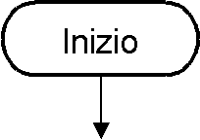
\includegraphics[scale=0.5]{Inizio.png} & Blocco di inizio \\
			\hline
			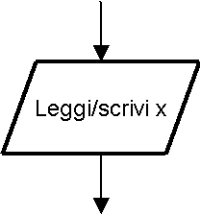
\includegraphics[scale=0.5]{Input.png} & Blocco di input o output \\
			\hline
			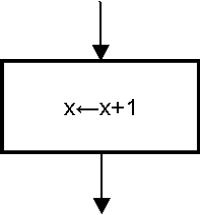
\includegraphics[scale=0.5]{Azione.png} & Blocco di assegnazione o operazione \\
			\hline
			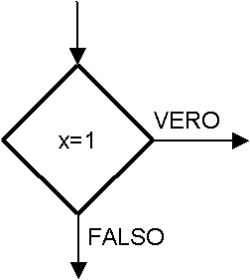
\includegraphics[scale=0.5]{Controllo.png} & Blocco di selezione \\
			\hline
			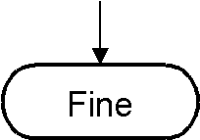
\includegraphics[scale=0.5]{Fine.png} & Blocco di fine \\
			\hline
		\end{tabular}
	\end{center}
	Le tre strutture fondamentali degli algoritmi possono essere descritte così con i diagrammi a blocchi. I blocchi vengono reppresentati uniti da frecce, che indicano il flusso di esecuzione dell'algoritmo.
	\subsubsection{Sequenza}
	I blocchi di apertura e chiusura dell’algoritmo hanno una sola sola freccia, rispettivamente uscente ed entrante, mentre i blocchi intermedi hanno generalmente una freccia entrante e una uscente
	\begin{figure}[h!]
		\centering
		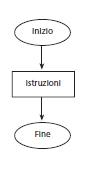
\includegraphics[scale=1]{Sequenza.png}
		\caption{Struttura generale della sequenza}
	\end{figure}
	\subsubsection{Selezione}
	Il blocco di controllo, nel caso più semplice, ha una freccia entrante e due uscenti, corrispondenti ai due valori di verità della condizione che viene valutata.
	\begin{figure}[h!]
		\centering
		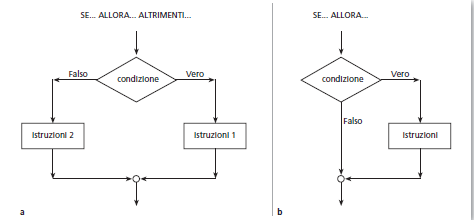
\includegraphics[scale=1]{Selezione.png}
		\caption{Struttura generale della selezione}
	\end{figure}
	\subsubsection{Iterazione}
	\begin{figure}[h!]
		\centering
		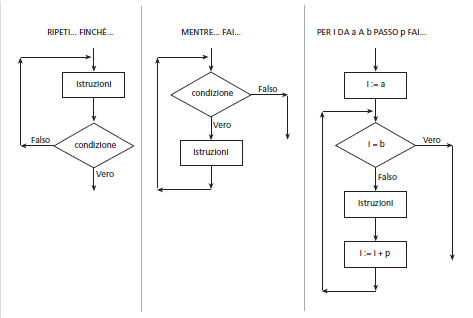
\includegraphics[scale=1]{Iterazione.png}
		\caption{Struttura generale dell'iterazione}
	\end{figure}



	\pagebreak
	
	\section{Esercizi}
	\subsection{Struttura di selezione}
	\begin{enumerate}
		\item Dati due numeri interi positivi N1 e N2, calcolare e visualizzare il numero massimo MAX tra i due
		\item Dati tre numeri interi positivi N1, N2, N3, calcolare e visualizzare il numero massimo MAX tra i tre
		\item Dati due numeri interi positivi N1 e N2, calcolare e visualizzare il numero minimo MIN tra i due
		\item Dati tre numeri interi positivi N1, N2, N3, calcolare e visualizzare il numero minimo MIN tra i tre
		\item Dato un numero intero positivo N, verificare se appartiene all'intervallo [4,10]
		\item Dato un numero intero positivo N, verificare se appartiene all'intervallo [4,10] o all'intervallo [15,20]
		\item Dato un numero intero positivo N, dire se è un multiplo di 2
		\item Dato un numero N, dire se è un multiplo di 7
		\item Dati due numeri N1, N2, dire se N1 è un multiplo di N2 o se N2 è un multiplo di N1
	\end{enumerate}

	\subsection{Struttura di iterazione}
	\begin{enumerate}
		\item Dato un numero N, generare e visualizzare in ordine crescente i numeri minori di N
		\item Dato un numero N, generare e visualizzare in ordine crescente i numeri dispari minori o uguali di N
		\item Dato un numero N, generare e visualizzare in ordine crescente i numeri pari minori o uguali di N
		\item Dato un numero N, generare e visualizzare in ordine decrescente i numeri minori di N
		\item Dati due numeri N1 e N2 (con N2 $>$ N1), generare e visualizzare in ordine crescente i numeri compresi tra N1 e N2
		\item Dati due numeri N1 e N2 (con N2 $>$ N1), generare e visualizzare in ordine decrescente i numeri compresi tra N1 e N2
		\item Dato un numero N, calcolare e visualizzare la somma dei numeri minori di N
		\item Dato un numero N, calcolare e visualizzare la somma dei numeri dispari minori di N
		\item Dati due numeri N1, N2, calcolare e visualizzare il prodotto dei due numeri tramite somma ripetuta
		\item Dato un numero N, calcolare e visualizzare il prodotto dei numeri minori di N
		\item Dati due numeri B,E, calcolare e visualizzare la potenza in base B ed esponente E, mediante il metodo delle moltiplicazioni ripetute
		\item Dato un numero N, verificare se N è un numero primo
	\end{enumerate}
	\subsection{Riassuntivi}
	\begin{enumerate}
		\item Dato un numero N, calcolare la differenza tra il quadrato del numero ed il numero stesso
		\item Dati due numeri N1, N2, verificare se uno dei è il quadrato dell'altro
		\item Dati quattro numeri N1, N2, N3, N4, verificare se costituiscono la proporzione N1:N2=N3:N4
		\item Data l'area A e la base B si un rettangolo, calcolarne il perimetro P
		\item Dato il perimetro P e l'altezza H di un rettangolo, calcolare l'area A
		\item Data la diagonale D ed un lato C di un rettangolo, calcolare l'area A del quadrato costruito sul lato maggiore
		\item Dati tre numeri A, B, C, determinare se A può essere l'ipotenusa di un triangolo rettangolo con i cateti uguali a B e C
		\item Data la misura di un angolo, verificare se è acuto, ottuso o retto
		\item Data una misura di tempo espressa in minuti M1, convertirla in ore H e minuti M
		\item Data una misura di tempo espressa in secondi S1, convertirla in ore H, minuti M e secondi S
		\item Date due misure espresse in ore e minuti, calcolare la differenza fra la prima e la seconda
		\item A fronte di un pagamento con una banconota da 100euro, calcolare il resto da fornire, usando solo banconote e monete esistenti
		\item Si conosce il prezzo di un oggetto O comprensivo di IVA (22\%), determina il prezzo netto
		\item Dato il prezzo P, se tale importo è maggiore di 300 allora fare uno sconto del 5\%
		\item Dato un numero N, trasforma e visualizza il corrispettivo codice binario
		\item Dato il numero di scatti telefonici N e sapendo che la bolletta del telefono viene calcolata nel seguente modo, calcola l'importo da pagare:
			\subitem minimo 7,5 euro per i primi 80 scatti
			\subitem più 0,6 euro/scatto per i successivi 60
			\subitem più 0,5 euro/scatto per i successivi 60
			\subitem più 0,4 euro/scatto per quelli oltre i 200
	\end{enumerate}

	\pagebreak
	
	\section{Esempi}
	\begin{figure}[h!]
		\centering
		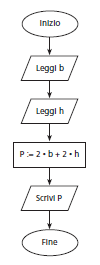
\includegraphics[scale=1]{Perimetro.png}
		\caption{Calcolo del perimetro di un rettangolo}
	\end{figure}
	\begin{figure}[h!]
		\centering
		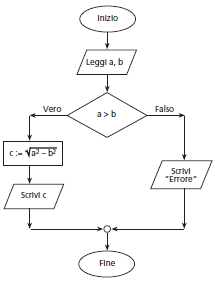
\includegraphics[scale=1]{Cateto.png}
		\caption{Calcolo del cateto di un triangolo rettangolo}
	\end{figure}
	\begin{figure}[h!]
		\centering
		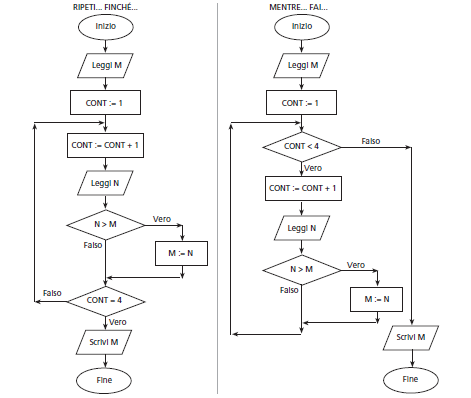
\includegraphics[scale=1]{Massimo4Numeri.png}
		\caption{Calcolo del massimo tra 4 numeri}
	\end{figure}
\end{document}